\documentclass{beamer}

\usepackage[utf8]{inputenc}
\usepackage{hyperref}
\hypersetup{
    colorlinks = true
    }
\usepackage{graphicx}
\usepackage{listings}

%Information to be included in the title page:
\title{Übersicht Programmierumgebungen}
\author{Mattias Schlenker}
\institute{TÖP Rabutz}
\date{ \today }

\begin{document}

\frame{\titlepage}

\begin{frame}
\frametitle{Open Source Hardware}
\begin{itemize}
\item Nahe Verwandtschaft zu ARM M0+ Boards von Arduino und Adafruit
\item Erweiterung um Motortreiber, MOSFET und bessere Anschlüsse
\item Open Source Hardware
\item Open Source Software 
\end{itemize}
\end{frame}


\begin{frame}
\frametitle{Programmierumgebung Arduino}

 \begin{figure}
  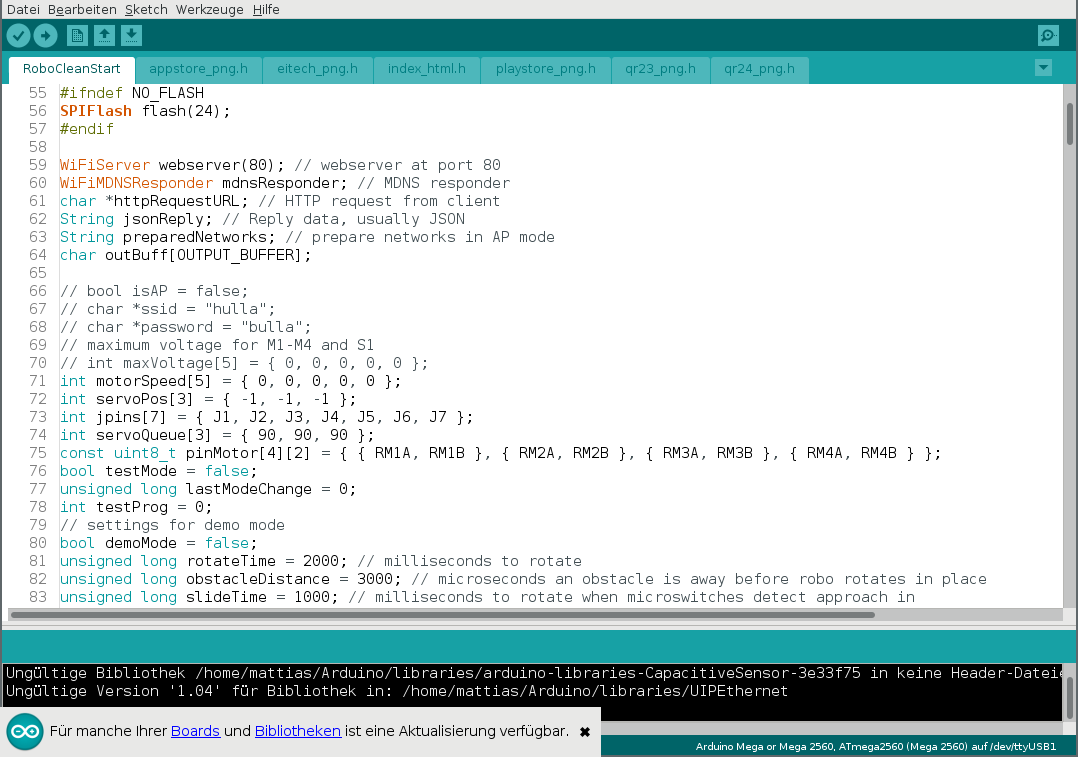
\includegraphics[width=8cm]{arduino.png}
  \caption{Arduino 1.8}
  \label{fig:arduino}
  \end{figure}
\end{frame}


\begin{frame}
\frametitle{Programmierumgebung Arduino}

Vorteile

\begin{itemize}
\item Unterstützung der kompletten verbauten Hardware
\item Sehr performant
\item Große Auswahl verfügbarer Erweiterungen
\end{itemize}

Nachteile 

\begin{itemize}
\item Höhere Einstiegsschwelle
\item Erfordert Installation
\end{itemize}

Altersempfehlung: Ab Klasse 7 aufwärts 

\end{frame}

\begin{frame}
\frametitle{Microsoft Makecode}

 \begin{figure}
  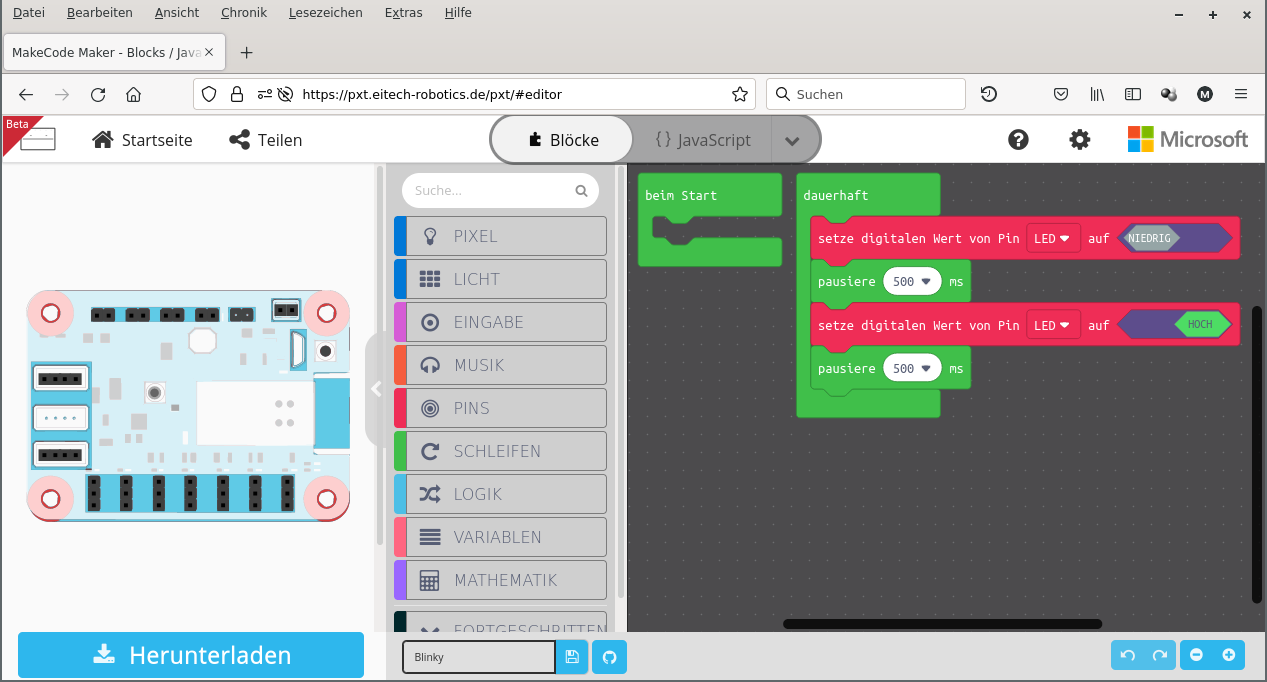
\includegraphics[width=10cm]{makecode.png}
  \caption{Makecode}
  \label{fig:makecode}
  \end{figure}

\end{frame}

\begin{frame}
\frametitle{Microsoft Makecode}

Vorteile

\begin{itemize}
\item Läuft im Browser
\item Sehr intuitiv 
\end{itemize}

Nachteile 

\begin{itemize}
\item Erfordert Internetverbindung (,,Self Hosting'' im LAN ist möglich)
\item WLAN-Modul (noch) nicht nutzbar 
\item MOSFET S1 nicht nutzbar
\end{itemize}

Altersempfehlung: Bis Klasse 8 

\end{frame}

\begin{frame}[fragile]

\frametitle{CircuitPython}

,,Work in Progress'' - Erwarte nutzbaren Port im November

\begin{lstlisting}[language=Python] 
import board
import digitalio
import time

led = digitalio.DigitalInOut(board.LED)
led.direction = digitalio.Direction.OUTPUT

while True:
    led.value = True
    time.sleep(0.5)
    led.value = False
    time.sleep(0.5)
\end{lstlisting} 
\end{frame}

\begin{frame}
\frametitle{CircuitPython}

Vorteile

\begin{itemize}
\item Sehr klare Syntax
\item Gute Dokumentation
\item Viele Erweiterungen
\item Kein Kompilieren erforderlich
\end{itemize}

Nachteile 

\begin{itemize}
\item Keine Interrupts
\item WLAN-Modul nicht nutzbar (unklar, ob es je nutzbar sein wird)
\end{itemize}

Altersempfehlung: Ab Klasse 6 

\end{frame}

\begin{frame}
\frametitle{Links und Kontakt}

\begin{itemize}
\item Makecode: pxt.eitech-robotics.com
\item Dokumentation: doc.schlenker.dk
\item Kontakt mattias@schlenker.dk
\end{itemize}

\end{frame}

\end{document}
